\documentclass[12pt,a4paper]{article}

\newcommand{\TETELNUMBER}{4}
\newcommand{\TETELTITLE}{Számelméleti algoritmusok}
\newcommand{\TETELSHORTTITLE}{Számelméleti algoritmusok, RSA}

\newcommand{\ZVTetelsorDataOnly}{}
\newcommand{\ZVTetelOne}{Adatok, adattípusok, adatműveletek és adatstruktúrák. Szám adattípus. Számrendszerek, konverziók. A logikai, halmaz, karakter, sztring absztrakt adattípusok és realizációjuk. A tömb (vektor, mátrix), rekord absztrakt adattípusok.}
\newcommand{\ZVTetelTwo}{Az algoritmus. Iteratív és rekurzív algoritmus. A számítógépes memória. Adat és program. Verem és procedúra. Az algoritmus lejegyzése. A folyamatábra és a pszeudokód. Elemi algoritmusok.}
\newcommand{\ZVTetelThree}{Strukturált programozás. Programgráf, valódi program, vezérlőgráf lebontása, strukturált program és annak formulája. Strukturált programgráf kialakítása, struktogram. Ciklikus bonyolultság és egyéb bonyolultsági tételek.}
\newcommand{\ZVTetelFour}{Számelméleti algoritmusok. Legnagyobb közös osztó, euklideszi és kibővített euklideszi algoritmus, lineáris kongruencia egyenletek. Multiplikatív inverz, moduláris hatványozás, Fermat prímteszt. RSA.}
\newcommand{\ZVTetelFive}{Rendezések: Beszúró rendezés. Az ,,Oszd meg és uralkodj!'' elv. Összefésülő rendezés. Gyors rendezés. Buborék rendezés. Shell rendezés. Minimum kiválasztásos rendezés. Négyzetes rendezés. Lineáris idejű rendezések: leszámláló rendezés, számjegyes rendezés. Időelemzéseik. Az összehasonlító rendezések időtétele.}
\newcommand{\ZVTetelSix}{Gráfalgoritmusok. Szélességi keresés. Mélységi keresés. Topologikus rendezés. Optimumfeladatok fákon (minimális feszítőfák, Kruskal- és Prim-algoritmus). Legrövidebb utak meghatározása (Dijkstra-algoritmus, Bellman--Ford-algoritmus, Floyd--Warshall-algoritmus).}
\newcommand{\ZVTetelSeven}{A párhuzamos algoritmusok alapfogalmai, PRAM modell, hatékonysági mértékek (munka, költség, gyorsítás, hatékonyság). Párhuzamos végrehajtás ábrázolási módjai. Komplexitás becslése, párhuzamos komplexitás. Amdahl törvénye. Pipeline párhuzamosítás, Lost update probléma bemutatása és megoldása.}
\newcommand{\ZVTetelEight}{Aggregáció, redukció, prefixszámítás párhuzamosítási lehetőségei. \texttt{CREW\_PREFIX}, \texttt{EREW\_PREFIX} és \texttt{OPTIMAL\_PREFIX} algoritmusok bemutatása. Összefésülő rendezés párhuzamosítási módja.}
\newcommand{\ZVTetelNine}{A busz, gyűrű, rács, tórusz, hiperkocka és fa topológiák bemutatása, csomópontok közötti távolságok jellemzése. A CSP, Publish--Subscribe és az Aktor modell. Az aszinkron programozás elemei: async, await kulcsszavak használata, coroutine-ok.}
\newcommand{\ZVTetelTen}{A Turing-gép fogalma, működése. A RAM-gép. Boole-függvények és logikai hálózatok.}
\newcommand{\ZVTetelEleven}{Algoritmikus eldönthetőség. Church-tézis. Rekurzív és rekurzívan felsorolható nyelvek, rekurzív illetve parciálisan rekurzív függvények. Nevezetes nyelvek (Az R, Re, coR, coRE nyelvosztályok és ezek kapcsolata) és bonyolultságuk. Algoritmikusan eldönthetetlen problémák. Polinomiális idejű algoritmusok.}
\newcommand{\ZVTetelTwelve}{Nemdeterminisztikus Turing-gépek, az NP és a coNP nyelvosztály. Példák NP-beli nyelvekre. A tanú-tétel. Nemdeterminisztikus algoritmusok bonyolultsága. NP-teljesség, Cook-tétel. Néhány NP-teljes probléma, Cook--Levin-tétel.}
\newcommand{\ZVTetelThirteen}{A Java programozási nyelv története, alapvető jellemzői. Egy Java program szerkezete (csomagok és fordítási egységek). Az objektumorientált programtervezés alapelveinek felsorolása. Objektumok tárolása és élettartama. Szemétgyűjtő mechanizmus. Kivételkezelés.}
\newcommand{\ZVTetelFourteen}{Az egységbezárás és az információrejtés objektumorientált alapelvek megvalósítása. Osztálydefiníció és példányosítás. Osztályszintű és példányszintű tagok, konstansok. Hozzáférési kategóriák és használatuk. Hivatkozás az osztály tagjaira.}
\newcommand{\ZVTetelFifteen}{Az öröklődés és a polimorfizmus objektumorientált alapelvek megvalósítása. Öröklődés szabályai, metódusok túlterhelése és felüldefiniálása. A referencia statikus és dinamikus típusa. Absztrakt osztály és interfész szerepe, összehasonlítása.}
\newcommand{\ZVTetelSixteen}{Az operációs rendszerbeli folyamat (processz) fogalma. Folyamatkontextus. A fonál (szál) fogalma. A processzállapotok, állapotváltások, processz futási módok. Taszk- és fonálállapotok, állapotátmenetek.}
\newcommand{\ZVTetelSeventeen}{A memóriamenedzselés feladatai. Memória mint erőforrás. Címleképzés fajtái. Lapozós virtuális memóriamenedzselés működése. Allokálás, nyilvántartás, címleképzés. Laphiba fogalma, kezelése, kilapozási stratégiák. Előnyök, hátrányok.}
\newcommand{\ZVTetelEighteen}{Fájlrendszer-megvalósítási feladatok. Jegyzékszerkezetek. Szabadblokk-menedzselési lehetőségek. Fájlattribútum-rögzítési lehetőségek (ezen belül a fájltestet képező blokkok rögzítési lehetőségei).}
\newcommand{\ZVTetelNineteen}{Relációs adatmodell, relációs struktúra és integritási feltételek. ER modell elemei jelentése és jelölése. Az ER modell konverziója relációs modellre. Relációs adatmodell műveleti része, relációs algebra.}
\newcommand{\ZVTetelTwenty}{Az SQL szabvány relációs adatbázis kezelő nyelv bemutatása, a DDL (objektum létrehozás, megszüntetés és szerkezet módosítás), DML (rekord felvitel, törlés és módosítás), DCL és a SELECT utasítások áttekintése és használata. Beágyazott SELECT használata. A relációs algebra műveleteinek megvalósítása SQL-ben.}
\newcommand{\ZVTetelTwentyOne}{Adatkezelés és adatbáziskezelés alapfogalmai, fileszervezési módszerek, B-fa index; adatbázis architektúra; A normalizálás szerepe a relációs adatbázis kezelésben. Redundancia oka és a megszüntetés lépései. Normálformák. Dekompozíció célja és szabályai, tételei.}
\newcommand{\ZVTetelTwentyTwo}{Számítógép-hálózatokhoz kötődő alapfogalmak és az ISO--OSI hivatkozási modell: topológia és méret szerinti osztályozásuk. Kapcsolástechnika szerinti osztályozásuk (vonalkapcsolás, üzenetkapcsolás, csomagkapcsolás és virtuális vonalkapcsolás). Az ISO--OSI hivatkozási modell szerkezete, rétegei és azok főbb funkciói.}
\newcommand{\ZVTetelTwentyThree}{A számítógép-hálózatok ISO--OSI hivatkozási modell adatkapcsolati rétegének közeghozzáférési alrétege: A főbb csatorna-megosztási osztályok (statikus-dinamikus, dinamikus versengő-determinisztikus) bemutatása és azok összevetése. Az IEEE 802.3 és az Ethernet (CSMA/CD) keretformátum, MAC címek, támogatott közegek és sebességek bemutatása, működés duplex csatorna esetén. Az IEEE 802.11 WLAN általános felépítése, az Access Point (AP) főbb funkciói. Az alkalmazott közeghozzáférési módszer (CSMA/CA), Distributed Coordination Function (DCF) és Point Coordination Function (PCF) üzemmódok.}
\newcommand{\ZVTetelTwentyFour}{A TCP/IP protokollszövet és az Internet. Az Internet hivatkozási modell (DoD) és az ISO--OSI hivatkozási modell összevetése. A TCP/IP protokollszövet főbb részei (ARP, RARP, IP, ICMP, TCP, UDP) és azok funkciói. Az internetes címzés és címosztályok: IPv4-címosztályok, maszk, subnet, supernet, osztály nélküli címzés (CIDR -- Classless Inter-Domain Routing) és változó alhálózat-méretek (VLSM -- Variable Length Subnet Mask), címek kiosztása, lokális címek és címfordítás (NAT). IPv6-címek, IPv6-címtípusok (unicast, multicast, anycast; link local, unique local, aggregatable global unicast address).}
\newcommand{\ZVTetelTwentyFive}{Szoftvertechnológia és a szoftverfolyamat fogalma. A szoftverfolyamat-fázisok részletes bemutatása: szoftverspecifikáció, tervezés, implementáció, validáció és evolúció. Az evolúciós modell ismertetése.}
\newcommand{\ZVTetelTwentySix}{Szoftverkövetelmény fogalma és osztályozásai. Követelmények általános problémái. Követelményfeltárás és -elemzés folyamata. Vezérlési stílusok.}
\newcommand{\ZVTetelTwentySeven}{UML diagramok bemutatása: Use case és osztálydiagram. A szekvenciadiagram. Komponensdiagram.}

\newcommand{\ZVTetelKiiras}[1]{%
  \ifcase#1\relax
  \or \ZVTetelOne
  \or \ZVTetelTwo
  \or \ZVTetelThree
  \or \ZVTetelFour
  \or \ZVTetelFive
  \or \ZVTetelSix
  \or \ZVTetelSeven
  \or \ZVTetelEight
  \or \ZVTetelNine
  \or \ZVTetelTen
  \or \ZVTetelEleven
  \or \ZVTetelTwelve
  \or \ZVTetelThirteen
  \or \ZVTetelFourteen
  \or \ZVTetelFifteen
  \or \ZVTetelSixteen
  \or \ZVTetelSeventeen
  \or \ZVTetelEighteen
  \or \ZVTetelNineteen
  \or \ZVTetelTwenty
  \or \ZVTetelTwentyOne
  \or \ZVTetelTwentyTwo
  \or \ZVTetelTwentyThree
  \or \ZVTetelTwentyFour
  \or \ZVTetelTwentyFive
  \or \ZVTetelTwentySix
  \or \ZVTetelTwentySeven
  \fi
}

\newcommand{\ZVTetelsorList}{%
\begin{enumerate}[leftmargin=7mm,label=\arabic*.,itemsep=2pt,topsep=2pt,parsep=0pt]
  \item \ZVTetelOne
  \item \ZVTetelTwo
  \item \ZVTetelThree
  \item \ZVTetelFour
  \item \ZVTetelFive
  \item \ZVTetelSix
  \item \ZVTetelSeven
  \item \ZVTetelEight
  \item \ZVTetelNine
  \item \ZVTetelTen
  \item \ZVTetelEleven
  \item \ZVTetelTwelve
  \item \ZVTetelThirteen
  \item \ZVTetelFourteen
  \item \ZVTetelFifteen
  \item \ZVTetelSixteen
  \item \ZVTetelSeventeen
  \item \ZVTetelEighteen
  \item \ZVTetelNineteen
  \item \ZVTetelTwenty
  \item \ZVTetelTwentyOne
  \item \ZVTetelTwentyTwo
  \item \ZVTetelTwentyThree
  \item \ZVTetelTwentyFour
  \item \ZVTetelTwentyFive
  \item \ZVTetelTwentySix
  \item \ZVTetelTwentySeven
\end{enumerate}%
}


\newcommand{\tetelsorrow}[2]{\textbf{#1.} & #2\tabularnewline}

\newcommand{\tetelsorpageone}{%
\begin{tabularx}{\textwidth}{|>{\raggedleft\bfseries}p{8mm}@{\hspace{5mm}}>{\raggedright\arraybackslash}X|}
\hline
\tetelsorrow{1}{\ZVTetelOne}
\tetelsorrow{2}{\ZVTetelTwo}
\tetelsorrow{3}{\ZVTetelThree}
\hline
\tetelsorrow{4}{\ZVTetelFour}
\tetelsorrow{5}{\ZVTetelFive}
\tetelsorrow{6}{\ZVTetelSix}
\hline
\tetelsorrow{7}{\ZVTetelSeven}
\tetelsorrow{8}{\ZVTetelEight}
\tetelsorrow{9}{\ZVTetelNine}
\hline
\tetelsorrow{10}{\ZVTetelTen}
\tetelsorrow{11}{\ZVTetelEleven}
\tetelsorrow{12}{\ZVTetelTwelve}
\hline
\end{tabularx}%
}

\newcommand{\tetelsorpagetwo}{%
\begin{tabularx}{\textwidth}{|>{\raggedleft\bfseries}p{8mm}@{\hspace{5mm}}>{\raggedright\arraybackslash}X|}
\hline
\tetelsorrow{13}{\ZVTetelThirteen}
\tetelsorrow{14}{\ZVTetelFourteen}
\tetelsorrow{15}{\ZVTetelFifteen}
\hline
\tetelsorrow{16}{\ZVTetelSixteen}
\tetelsorrow{17}{\ZVTetelSeventeen}
\tetelsorrow{18}{\ZVTetelEighteen}
\hline
\tetelsorrow{19}{\ZVTetelNineteen}
\tetelsorrow{20}{\ZVTetelTwenty}
\tetelsorrow{21}{\ZVTetelTwentyOne}
\hline
\tetelsorrow{22}{\ZVTetelTwentyTwo}
\tetelsorrow{23}{\ZVTetelTwentyThree}
\tetelsorrow{24}{\ZVTetelTwentyFour}
\hline
\tetelsorrow{25}{\ZVTetelTwentyFive}
\tetelsorrow{26}{\ZVTetelTwentySix}
\tetelsorrow{27}{\ZVTetelTwentySeven}
\hline
\end{tabularx}%
}

\ifdefined\ZVTetelsorDataOnly
\expandafter\endinput
\fi

\documentclass[10pt,a4paper]{article}
\newcommand{\ZVHEADERLEFT}{Záróvizsga tételek}
\newcommand{\ZVHEADERRIGHT}{Programtervező informatikus BSc}
\usepackage{fontspec}
\usepackage{geometry}
\usepackage{microtype}
\usepackage{xcolor}
\usepackage{amsmath,amssymb,mathtools}
\usepackage{booktabs,longtable,tabularx,array,multirow}
\usepackage{enumitem}
\usepackage{hyperref}
\usepackage{fancyhdr}
\usepackage{titlesec}
\usepackage{listings}
\usepackage[most]{tcolorbox}
\usepackage{tikz}
\usetikzlibrary{positioning,shapes.geometric,shapes.misc,arrows.meta,decorations.pathreplacing}
\usepackage{caption}

\setlength{\headheight}{16pt}
\emergencystretch=2em
\renewcommand{\contentsname}{Tartalom}

% Fontbeallitasok: ha a DejaVu fontok nincsenek telepitve,
% akkor automatikusan a MiKTeX/TeX Live alap Latin Modern fontjaira valtunk.
\IfFontExistsTF{DejaVu Serif}{\setmainfont{DejaVu Serif}}{\setmainfont{Latin Modern Roman}}
\IfFontExistsTF{DejaVu Sans}{\setsansfont{DejaVu Sans}}{\setsansfont{Latin Modern Sans}}
\IfFontExistsTF{DejaVu Sans Mono}{\setmonofont{DejaVu Sans Mono}}{\setmonofont{Latin Modern Mono}}

\geometry{left=25mm,right=25mm,top=24mm,bottom=27mm}

\hypersetup{
  colorlinks=true,
  linkcolor=blue!45!black,
  urlcolor=blue!55!black,
  pdftitle={Zarovizsga tetel},
  pdfauthor={Baba Levente - tanulasi segedanyag}
}

\definecolor{accent}{HTML}{1F4E79}
\definecolor{lightaccent}{HTML}{EAF2F8}
\definecolor{warnbg}{HTML}{FFF4E5}
\definecolor{codebg}{HTML}{F7F7F7}

\tikzset{
  flow/.style={draw, rounded corners, align=center, minimum width=21mm, minimum height=8mm, fill=lightaccent},
  pred/.style={draw, diamond, aspect=2, align=center, inner sep=1pt, fill=warnbg},
  merge/.style={draw, circle, inner sep=1.2pt, fill=black!8},
  terminator/.style={draw, rounded corners=4mm, align=center, minimum width=20mm, minimum height=8mm, fill=black!5},
  arrow/.style={->, >=stealth, thick},
  zvflowstart/.style={draw, rounded rectangle, minimum width=2.3cm, minimum height=0.7cm, align=center},
  zvflowprocess/.style={draw, rectangle, minimum width=2.7cm, minimum height=0.7cm, align=center},
  zvflowdecision/.style={draw, diamond, aspect=2.2, minimum width=2.8cm, minimum height=0.8cm, align=center}
}


\titleformat{\section}{\Large\bfseries\sffamily\color{accent}}{\thesection.}{0.6em}{}
\titleformat{\subsection}{\large\bfseries\sffamily\color{accent}}{\thesubsection.}{0.6em}{}
\titleformat{\subsubsection}{\normalsize\bfseries\sffamily\color{accent}}{\thesubsubsection.}{0.6em}{}

\setlist[itemize]{topsep=3pt,itemsep=2pt,parsep=0pt,leftmargin=1.4em}
\setlist[enumerate]{topsep=3pt,itemsep=2pt,parsep=0pt,leftmargin=1.6em}
\setlength{\parindent}{0pt}
\setlength{\parskip}{6pt}
\renewcommand{\arraystretch}{1.25}
\newcolumntype{L}[1]{>{\raggedright\arraybackslash}p{#1}}
\renewcommand{\tabularxcolumn}[1]{>{\raggedright\arraybackslash}p{#1}}

\providecommand{\ZVHEADERLEFT}{\TETELNUMBER. tétel}
\providecommand{\ZVHEADERRIGHT}{\TETELSHORTTITLE}

\pagestyle{fancy}
\fancyhf{}
\lhead{\ZVHEADERLEFT}
\rhead{\ZVHEADERRIGHT}
\cfoot{\thepage}

\lstdefinelanguage{pseudocode}{
  morekeywords={IF,THEN,ELSE,WHILE,DO,FOR,TO,DOWNTO,REPEAT,UNTIL,RETURN,CALL,INPUT,OUTPUT,AND,OR,NOT,TRUE,FALSE},
  sensitive=true,
  morecomment=[l]{//}
}

\lstdefinestyle{code}{
  basicstyle=\ttfamily\small,
  backgroundcolor=\color{codebg},
  frame=single,
  rulecolor=\color{black!15},
  columns=fullflexible,
  keepspaces=true,
  breaklines=true,
  tabsize=2,
  showstringspaces=false,
  numbers=left,
  numberstyle=\tiny\color{black!55},
  numbersep=7pt,
  xleftmargin=2.2em,
  framexleftmargin=1.7em,
  captionpos=b
}

\lstdefinestyle{pseudo}{
  style=code,
  language=pseudocode,
  keywordstyle=\bfseries\color{accent!85!black},
  commentstyle=\itshape\color{black!55}
}

\lstdefinestyle{csource}{
  style=code,
  language=C,
  keywordstyle=\bfseries\color{accent!85!black},
  commentstyle=\itshape\color{black!55},
  stringstyle=\color{orange!70!black}
}

\lstset{style=code}
\renewcommand{\lstlistingname}{Kódrészlet}
\renewcommand{\lstlistlistingname}{Kódrészletek}
\newcommand{\zvcode}[2][]{\lstinputlisting[style=code,#1]{#2}}
\newcommand{\zvpseudocode}[2][]{\lstinputlisting[style=pseudo,#1]{#2}}
\newcommand{\zvccode}[2][]{\lstinputlisting[style=csource,#1]{#2}}

\newtcolorbox{summarybox}{
  enhanced,
  colback=lightaccent,
  colframe=accent!70!black,
  arc=2mm,
  boxrule=0.5pt,
  left=2mm,right=2mm,top=1mm,bottom=1mm
}

\newtcolorbox{warningbox}{
  enhanced,
  colback=warnbg,
  colframe=orange!70!black,
  arc=2mm,
  boxrule=0.5pt,
  left=2mm,right=2mm,top=1mm,bottom=1mm
}

\newcommand{\adt}[2]{\ensuremath{#1=(#2)}}
\newcommand{\set}[1]{\ensuremath{\{#1\}}}
\newcommand{\code}[1]{\texttt{#1}}
\newcommand{\base}[2]{\ensuremath{#1_{(#2)}}}
\newcommand{\addr}{\ensuremath{@}}


\providecommand{\TETELKIIRAS}{\TETELTITLE. \TETELTOPIC}
\providecommand{\ZVAUTHOR}{Baba Levente}
\providecommand{\ZVYEAR}{2026}
\providecommand{\ZVAID}{ChatGPT segítségével}

\newcommand{\makezvtitle}{%
\begin{titlepage}
  \centering
  \vspace*{18mm}
  {\Large\sffamily Programtervező Informatikus BSc\par}
  \vspace{1mm}
  {\large\sffamily \ZVYEAR-os záróvizsga tételek\par}
  \vspace{15mm}
  {\Huge\bfseries\sffamily \TETELNUMBER. tétel\par}
  \vspace{5mm}
  {\LARGE\bfseries\sffamily \TETELTITLE\par}
  \vspace{10mm}
  \begin{summarybox}
    \textbf{Tételkiírás:} \TETELKIIRAS
  \end{summarybox}
  \vfill
  {\large Készítette: \textbf{\ZVAUTHOR}\par}
  \vspace{2mm}
  {\large \ZVAID\par}
\end{titlepage}%
}

\newcommand{\zvfrontmatter}{%
  \sloppy
  \makezvtitle
  \tableofcontents
  \newpage
}

\begin{document}
\newgeometry{left=13mm,right=13mm,top=13mm,bottom=13mm}
\pagestyle{empty}
\setlength{\tabcolsep}{2.6pt}
\renewcommand{\arraystretch}{1.08}
\begin{center}
  {\Huge\bfseries Záróvizsga tételek\par}
  \vspace{2mm}
  {\Large\itshape Programtervező informatikus BSc\par}
\end{center}
\vspace{10mm}
{\fontsize{10.5}{12.2}\selectfont
\tetelsorpageone
}
\newpage
{\fontsize{10.5}{12.2}\selectfont
\tetelsorpagetwo
}
\end{document}

\newcommand{\TETELKIIRAS}{\ZVTetelKiiras{\TETELNUMBER}}

\usepackage{fontspec}
\usepackage{geometry}
\usepackage{microtype}
\usepackage{xcolor}
\usepackage{amsmath,amssymb,mathtools}
\usepackage{booktabs,longtable,tabularx,array,multirow}
\usepackage{enumitem}
\usepackage{hyperref}
\usepackage{fancyhdr}
\usepackage{titlesec}
\usepackage{listings}
\usepackage[most]{tcolorbox}
\usepackage{tikz}
\usetikzlibrary{positioning,shapes.geometric,shapes.misc,arrows.meta,decorations.pathreplacing}
\usepackage{caption}

\setlength{\headheight}{16pt}
\emergencystretch=2em
\renewcommand{\contentsname}{Tartalom}

% Fontbeallitasok: ha a DejaVu fontok nincsenek telepitve,
% akkor automatikusan a MiKTeX/TeX Live alap Latin Modern fontjaira valtunk.
\IfFontExistsTF{DejaVu Serif}{\setmainfont{DejaVu Serif}}{\setmainfont{Latin Modern Roman}}
\IfFontExistsTF{DejaVu Sans}{\setsansfont{DejaVu Sans}}{\setsansfont{Latin Modern Sans}}
\IfFontExistsTF{DejaVu Sans Mono}{\setmonofont{DejaVu Sans Mono}}{\setmonofont{Latin Modern Mono}}

\geometry{left=25mm,right=25mm,top=24mm,bottom=27mm}

\hypersetup{
  colorlinks=true,
  linkcolor=blue!45!black,
  urlcolor=blue!55!black,
  pdftitle={Zarovizsga tetel},
  pdfauthor={Baba Levente - tanulasi segedanyag}
}

\definecolor{accent}{HTML}{1F4E79}
\definecolor{lightaccent}{HTML}{EAF2F8}
\definecolor{warnbg}{HTML}{FFF4E5}
\definecolor{codebg}{HTML}{F7F7F7}

\tikzset{
  flow/.style={draw, rounded corners, align=center, minimum width=21mm, minimum height=8mm, fill=lightaccent},
  pred/.style={draw, diamond, aspect=2, align=center, inner sep=1pt, fill=warnbg},
  merge/.style={draw, circle, inner sep=1.2pt, fill=black!8},
  terminator/.style={draw, rounded corners=4mm, align=center, minimum width=20mm, minimum height=8mm, fill=black!5},
  arrow/.style={->, >=stealth, thick},
  zvflowstart/.style={draw, rounded rectangle, minimum width=2.3cm, minimum height=0.7cm, align=center},
  zvflowprocess/.style={draw, rectangle, minimum width=2.7cm, minimum height=0.7cm, align=center},
  zvflowdecision/.style={draw, diamond, aspect=2.2, minimum width=2.8cm, minimum height=0.8cm, align=center}
}


\titleformat{\section}{\Large\bfseries\sffamily\color{accent}}{\thesection.}{0.6em}{}
\titleformat{\subsection}{\large\bfseries\sffamily\color{accent}}{\thesubsection.}{0.6em}{}
\titleformat{\subsubsection}{\normalsize\bfseries\sffamily\color{accent}}{\thesubsubsection.}{0.6em}{}

\setlist[itemize]{topsep=3pt,itemsep=2pt,parsep=0pt,leftmargin=1.4em}
\setlist[enumerate]{topsep=3pt,itemsep=2pt,parsep=0pt,leftmargin=1.6em}
\setlength{\parindent}{0pt}
\setlength{\parskip}{6pt}
\renewcommand{\arraystretch}{1.25}
\newcolumntype{L}[1]{>{\raggedright\arraybackslash}p{#1}}
\renewcommand{\tabularxcolumn}[1]{>{\raggedright\arraybackslash}p{#1}}

\providecommand{\ZVHEADERLEFT}{\TETELNUMBER. tétel}
\providecommand{\ZVHEADERRIGHT}{\TETELSHORTTITLE}

\pagestyle{fancy}
\fancyhf{}
\lhead{\ZVHEADERLEFT}
\rhead{\ZVHEADERRIGHT}
\cfoot{\thepage}

\lstdefinelanguage{pseudocode}{
  morekeywords={IF,THEN,ELSE,WHILE,DO,FOR,TO,DOWNTO,REPEAT,UNTIL,RETURN,CALL,INPUT,OUTPUT,AND,OR,NOT,TRUE,FALSE},
  sensitive=true,
  morecomment=[l]{//}
}

\lstdefinestyle{code}{
  basicstyle=\ttfamily\small,
  backgroundcolor=\color{codebg},
  frame=single,
  rulecolor=\color{black!15},
  columns=fullflexible,
  keepspaces=true,
  breaklines=true,
  tabsize=2,
  showstringspaces=false,
  numbers=left,
  numberstyle=\tiny\color{black!55},
  numbersep=7pt,
  xleftmargin=2.2em,
  framexleftmargin=1.7em,
  captionpos=b
}

\lstdefinestyle{pseudo}{
  style=code,
  language=pseudocode,
  keywordstyle=\bfseries\color{accent!85!black},
  commentstyle=\itshape\color{black!55}
}

\lstdefinestyle{csource}{
  style=code,
  language=C,
  keywordstyle=\bfseries\color{accent!85!black},
  commentstyle=\itshape\color{black!55},
  stringstyle=\color{orange!70!black}
}

\lstset{style=code}
\renewcommand{\lstlistingname}{Kódrészlet}
\renewcommand{\lstlistlistingname}{Kódrészletek}
\newcommand{\zvcode}[2][]{\lstinputlisting[style=code,#1]{#2}}
\newcommand{\zvpseudocode}[2][]{\lstinputlisting[style=pseudo,#1]{#2}}
\newcommand{\zvccode}[2][]{\lstinputlisting[style=csource,#1]{#2}}

\newtcolorbox{summarybox}{
  enhanced,
  colback=lightaccent,
  colframe=accent!70!black,
  arc=2mm,
  boxrule=0.5pt,
  left=2mm,right=2mm,top=1mm,bottom=1mm
}

\newtcolorbox{warningbox}{
  enhanced,
  colback=warnbg,
  colframe=orange!70!black,
  arc=2mm,
  boxrule=0.5pt,
  left=2mm,right=2mm,top=1mm,bottom=1mm
}

\newcommand{\adt}[2]{\ensuremath{#1=(#2)}}
\newcommand{\set}[1]{\ensuremath{\{#1\}}}
\newcommand{\code}[1]{\texttt{#1}}
\newcommand{\base}[2]{\ensuremath{#1_{(#2)}}}
\newcommand{\addr}{\ensuremath{@}}


\providecommand{\TETELKIIRAS}{\TETELTITLE. \TETELTOPIC}
\providecommand{\ZVAUTHOR}{Baba Levente}
\providecommand{\ZVYEAR}{2026}
\providecommand{\ZVAID}{ChatGPT segítségével}

\newcommand{\makezvtitle}{%
\begin{titlepage}
  \centering
  \vspace*{18mm}
  {\Large\sffamily Programtervező Informatikus BSc\par}
  \vspace{1mm}
  {\large\sffamily \ZVYEAR-os záróvizsga tételek\par}
  \vspace{15mm}
  {\Huge\bfseries\sffamily \TETELNUMBER. tétel\par}
  \vspace{5mm}
  {\LARGE\bfseries\sffamily \TETELTITLE\par}
  \vspace{10mm}
  \begin{summarybox}
    \textbf{Tételkiírás:} \TETELKIIRAS
  \end{summarybox}
  \vfill
  {\large Készítette: \textbf{\ZVAUTHOR}\par}
  \vspace{2mm}
  {\large \ZVAID\par}
\end{titlepage}%
}

\newcommand{\zvfrontmatter}{%
  \sloppy
  \makezvtitle
  \tableofcontents
  \newpage
}


\begin{document}
\zvfrontmatter

\section{A tétel lényege és vizsgaszintű vázlata}

\begin{summarybox}
A tétel központi gondolata az, hogy több kriptográfiai és algoritmikai feladat visszavezethető egyszerű számelméleti műveletekre: oszthatóságra, maradékos osztásra, legnagyobb közös osztóra, kongruenciákra és moduláris hatványozásra. Ezek közül az RSA azért különösen jó összefoglaló példa, mert a kulcsgenerálás a kibővített euklideszi algoritmust, a titkosítás és visszafejtés pedig a moduláris hatványozást használja.
\end{summarybox}

A tétel vizsgán jól felépíthető a következő sorrendben:

\begin{enumerate}
  \item alapfogalmak: oszthatóság, prím, maradékos osztás, kongruencia;
  \item legnagyobb közös osztó, relatív prímek, lineáris kombináció;
  \item euklideszi algoritmus az lnko gyors kiszámítására;
  \item kibővített euklideszi algoritmus és a Bézout-együtthatók;
  \item lineáris kongruencia egyenletek és megoldhatósági feltétel;
  \item multiplikatív inverz modulo $n$ szerint;
  \item moduláris hatványozás négyzetre emeléssel és szorzással;
  \item Fermat-tétel és Fermat-féle prímteszt;
  \item RSA kulcsgenerálás, titkosítás, visszafejtés és a biztonsági alapgondolat.
\end{enumerate}

A legfontosabb vizsgamondat: a kibővített euklideszi algoritmus nemcsak azt adja meg, hogy mennyi $\operatorname{lnko}(a,b)$, hanem azt is, hogyan írható fel ez a legnagyobb közös osztó $a$ és $b$ egész lineáris kombinációjaként. Ez teszi lehetővé a lineáris kongruenciák, a multiplikatív inverz és az RSA titkos kitevőjének meghatározását.

\begin{center}
\begingroup
\setlength{\tabcolsep}{4pt}
\begin{longtable}{L{0.21\textwidth}L{0.35\textwidth}L{0.23\textwidth}L{0.10\textwidth}}
\toprule
Algoritmus & Feladat & Fő ötlet & Időigény röviden \\
\midrule
\endfirsthead
\toprule
Algoritmus & Feladat & Fő ötlet & Időigény röviden \\
\midrule
\endhead
Euklideszi algoritmus & $\operatorname{lnko}(a,b)$ meghatározása. & $\operatorname{lnko}(a,b)=\operatorname{lnko}(b,a\bmod b)$, amíg a maradék nulla nem lesz. & $O(\log b)$ \\
Kibővített euklideszi algoritmus & $d=\operatorname{lnko}(a,b)$ és $x,y$ keresése úgy, hogy $d=ax+by$. & Az euklideszi lépésekhez az együtthatókat is visszaszámolja. & $O(\log b)$ \\
Lineáris kongruencia megoldása & $ax\equiv b\pmod n$ megoldásai. & Először $d=\operatorname{lnko}(a,n)$; megoldás pontosan akkor van, ha $d\mid b$. & $O(\log n+d)$ \\
Multiplikatív inverz & $a^{-1}\pmod n$ meghatározása. & Az $ax\equiv1\pmod n$ kongruencia egyedi alapmegoldása, ha $\operatorname{lnko}(a,n)=1$. & $O(\log n)$ \\
Moduláris hatványozás & $a^b\bmod n$ gyors kiszámítása. & Négyzetre emelés és szorzás a kitevő bináris alakja alapján. & $O(\log b)$ szorzás \\
Fermat-prímteszt & Gyors valószínűségi prímszűrés. & Prím $p$ esetén $a^{p-1}\equiv1\pmod p$ minden $1\leq a<p$ esetén. & $O(\log n)$ moduláris hatványozás \\
RSA & Nyilvános kulcsú titkosítás és visszafejtés. & Kulcsgenerálás prímekkel, titkosítás és dekódolás moduláris hatványozással. & kulcsméretfüggő \\
\bottomrule
\end{longtable}
\endgroup

\end{center}

\section{Számelméleti alapfogalmak}

\subsection{Oszthatóság és maradékos osztás}

Azt mondjuk, hogy a $d$ egész szám \textbf{osztja} az $a$ egész számot, ha létezik olyan $k\in\mathbb{Z}$, amelyre

\[
a=k\cdot d.
\]

Jelölése: $d\mid a$. Ha $d\mid a$, akkor $d$ az $a$ osztója, $a$ pedig $d$ többszöröse. Ha $d\nmid a$, akkor $d$ nem osztja $a$-t.

A \textbf{maradékos osztás tétele} szerint ha $a\in\mathbb{Z}$ és $n\in\mathbb{Z}^{+}$, akkor egyértelműen léteznek olyan $q,r\in\mathbb{Z}$ számok, hogy

\[
a=q\cdot n+r,\qquad 0\leq r<n.
\]

Itt $q$ a hányados, $r$ a maradék. Programozási jelöléssel:

\[
q=a\operatorname{ div }n,\qquad r=a\bmod n.
\]

Példa:

\[
37=5\cdot 7+2,
\]

ezért $37\operatorname{ div }7=5$ és $37\bmod7=2$.

\subsection{Prímszám és összetett szám}

Egy $p>1$ egész szám \textbf{prímszám}, ha pozitív osztói csak $1$ és $p$. Ha egy $n>1$ egész szám nem prím, akkor \textbf{összetett}. Például:

\[
2,3,5,7,11,13
\]

prímek, míg

\[
4=2\cdot2,\qquad 12=3\cdot4
\]

összetett számok.

A prímek az RSA-ban kulcsszerepet kapnak, mert két nagy prím szorzatát könnyű kiszámítani, de a szorzat prímtényezőkre bontása nagy számok esetén nehéz feladat.

\subsection{Kongruencia}

Két egész szám kongruens modulo $n$ szerint, ha azonos maradékot adnak $n$-nel osztva, vagy ekvivalensen $n$ osztja a különbségüket:

\[
a\equiv b\pmod n \quad\Longleftrightarrow\quad n\mid(a-b).
\]

Például:

\[
17\equiv5\pmod{12},
\]

mert $17-5=12$, és $12\mid12$. Ugyanez maradékokkal nézve: $17\bmod12=5$ és $5\bmod12=5$.

A kongruenciákon a szokásos műveletek jelentős része elvégezhető. Ha $a\equiv b\pmod n$ és $c\equiv d\pmod n$, akkor:

\[
a+c\equiv b+d\pmod n,
\]

\[
a-c\equiv b-d\pmod n,
\]

\[
a\cdot c\equiv b\cdot d\pmod n.
\]

Az osztás viszont nem mindig végezhető el egyszerűen. Modulo $n$ szerint csak akkor tudunk egy számmal osztani, ha annak létezik multiplikatív inverze modulo $n$ szerint.

\section{Legnagyobb közös osztó}

\subsection{Közös osztó és lnko}

Egy $d$ egész szám az $a$ és $b$ egészek \textbf{közös osztója}, ha

\[
d\mid a \quad\text{és}\quad d\mid b.
\]

Az $a$ és $b$ számok \textbf{legnagyobb közös osztója} az a legnagyobb nemnegatív egész szám, amely mindkettőt osztja. Jelölése:

\[
\operatorname{lnko}(a,b).
\]

Például:

\[
\operatorname{lnko}(36,60)=12.
\]

Ha $\operatorname{lnko}(a,b)=1$, akkor $a$ és $b$ \textbf{relatív prímek}. Ez nem azt jelenti, hogy külön-külön prímek, hanem azt, hogy nincs $1$-nél nagyobb közös osztójuk. Például $8$ és $15$ relatív prímek, pedig egyik sem prím.

\subsection{Lineáris kombináció és Bézout-azonosság}

Az $s$ egész szám az $a$ és $b$ egészek egész lineáris kombinációja, ha léteznek $x,y\in\mathbb{Z}$ együtthatók úgy, hogy

\[
s=x\cdot a+y\cdot b.
\]

A legfontosabb tétel szerint a legnagyobb közös osztó is felírható ilyen alakban:

\[
\operatorname{lnko}(a,b)=x\cdot a+y\cdot b.
\]

Ezt szokás Bézout-azonosságnak nevezni. A $x$ és $y$ együtthatókat nem az egyszerű euklideszi algoritmus, hanem a kibővített euklideszi algoritmus adja meg.

\begin{warningbox}
A Bézout-együtthatók általában nem egyértelműek. A kibővített euklideszi algoritmus egy megfelelő együtthatópárt ad vissza, de ugyanahhoz az lnko-hoz több különböző lineáris kombináció is tartozhat.
\end{warningbox}

\subsection{Az lnko alapvető tulajdonságai}

Az lnko használatánál a következő tulajdonságok különösen fontosak:

\begin{itemize}
  \item $\operatorname{lnko}(a,b)=\operatorname{lnko}(b,a)$;
  \item $\operatorname{lnko}(a,0)=|a|$;
  \item $\operatorname{lnko}(a,b)=\operatorname{lnko}(|a|,|b|)$;
  \item ha $d=\operatorname{lnko}(a,b)$, akkor $d$ osztja $a$ és $b$ minden egész lineáris kombinációját;
  \item ha $\operatorname{lnko}(a,n)=1$, akkor $a$-nak létezik inverze modulo $n$ szerint.
\end{itemize}

\section{Euklideszi algoritmus}

\subsection{A redukciós ötlet}

Az euklideszi algoritmus alapja az a megfigyelés, hogy a legnagyobb közös osztó nem változik, ha a nagyobb szám helyett annak a kisebb számmal vett maradékát használjuk:

\[
\operatorname{lnko}(a,b)=\operatorname{lnko}(b,a\bmod b),\qquad b\neq0.
\]

Indoklás röviden: ha $a=q\cdot b+r$, akkor $r=a-qb$. Minden közös osztó, amely osztja $a$-t és $b$-t, osztja $r$-t is. Fordítva, minden közös osztó, amely osztja $b$-t és $r$-t, osztja $a=qb+r$-t is. Ezért a közös osztók halmaza ugyanaz, így a legnagyobb közös osztó is ugyanaz.

\subsection{Pszeudókód}

\zvpseudocode[caption={Euklideszi algoritmus},label={lst:zv04_euklideszi_algoritmus}]{src/code/zv04_euklideszi_algoritmus.pseudo}

Az algoritmus minden lépésben csökkenti a második argumentumot, mert $0\leq a\bmod b<b$. Emiatt véges sok lépés után eljutunk a $b=0$ állapotba. Ekkor az lnko az aktuális $a$ érték.

\begin{center}
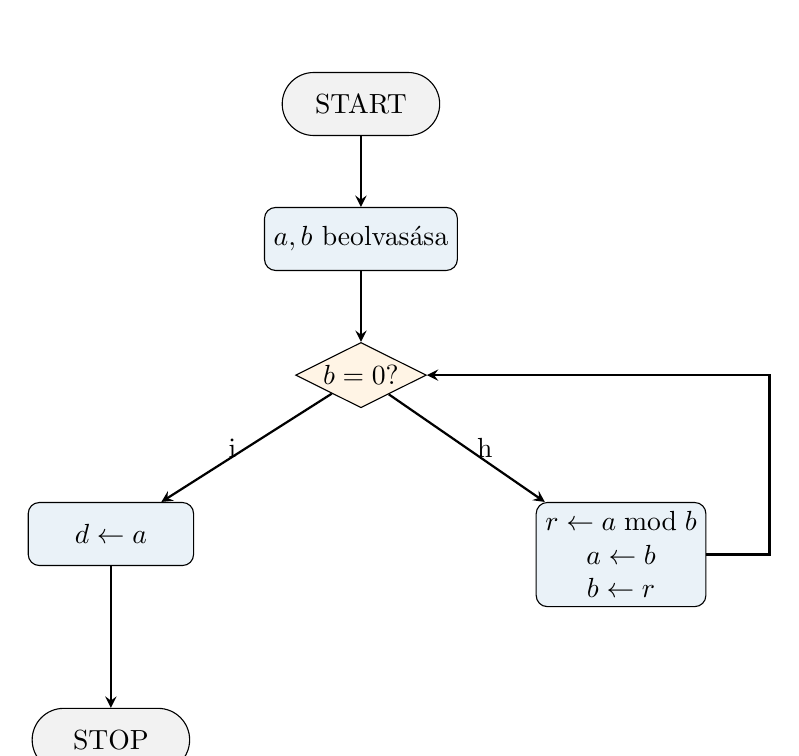
\begin{tikzpicture}[node distance=9mm]
  \node[terminator] (start) {START};
  \node[flow, below=of start] (input) {$a,b$ beolvasása};
  \node[pred, below=of input] (test) {$b=0$?};
  \node[flow, below left=14mm and 17mm of test] (return) {$d\leftarrow a$};
  \node[flow, below right=14mm and 18mm of test] (step) {$r\leftarrow a\bmod b$\\$a\leftarrow b$\\$b\leftarrow r$};
  \node[terminator, below=18mm of return] (stop) {STOP};
  \draw[arrow] (start) -- (input);
  \draw[arrow] (input) -- (test);
  \draw[arrow] (test) -- node[left] {i} (return);
  \draw[arrow] (return) -- (stop);
  \draw[arrow] (test) -- node[right] {h} (step);
  \draw[arrow] (step.east) -- ++(8mm,0) |- (test.east);
\end{tikzpicture}
\end{center}


\subsection{Példa: $\operatorname{lnko}(3604,3332)$}

\[
3604=1\cdot3332+272,
\]

\[
3332=12\cdot272+68,
\]

\[
272=4\cdot68+0.
\]

Tehát:

\[
\operatorname{lnko}(3604,3332)=68.
\]

\subsection{Időigény}

Az euklideszi algoritmus nagyon hatékony. Ha $a>b\geq0$, akkor a lépésszám $O(\log b)$ nagyságrendű, ha az aritmetikai műveleteket konstans idejűnek tekintjük. A legrosszabb esetek a szomszédos Fibonacci-számok környékén adódnak, de még ilyenkor is logaritmikus számú maradékos osztás elegendő.

\section{Kibővített euklideszi algoritmus}

\subsection{Mit bővít ki?}

Az egyszerű euklideszi algoritmus csak az lnko értékét adja meg. A \textbf{kibővített euklideszi algoritmus} ezen felül olyan $x$ és $y$ egész számokat is kiszámít, amelyekre

\[
\operatorname{lnko}(a,b)=a\cdot x+b\cdot y.
\]

Ezeket az $x$ és $y$ értékeket Bézout-együtthatóknak nevezzük.

\subsection{Rekurzív összefüggés}

Legyen

\[
d=\operatorname{lnko}(b,a\bmod b).
\]

Ha a rekurzív hívásból tudjuk, hogy

\[
d=b\cdot x_1+(a\bmod b)\cdot y_1,
\]

akkor mivel

\[
a\bmod b=a-\left\lfloor\frac{a}{b}\right\rfloor b,
\]

kapjuk:

\[
\begin{aligned}
d &= b\cdot x_1+\left(a-\left\lfloor\frac{a}{b}\right\rfloor b\right)y_1 \\
  &= a\cdot y_1+b\cdot\left(x_1-\left\lfloor\frac{a}{b}\right\rfloor y_1\right).
\end{aligned}
\]

Ezért az új együtthatók:

\[
x=y_1,
\]

\[
y=x_1-\left\lfloor\frac{a}{b}\right\rfloor y_1.
\]

\subsection{Pszeudókód}

\zvpseudocode[caption={Kibővített euklideszi algoritmus},label={lst:zv04_kibovitett_euklideszi_algoritmus}]{src/code/zv04_kibovitett_euklideszi_algoritmus.pseudo}

A visszatérési érték jelentése:

\[
(d,x,y),\qquad d=\operatorname{lnko}(a,b),\qquad d=ax+by.
\]

\subsection{Példa}

Az előző példában:

\[
\operatorname{lnko}(3604,3332)=68.
\]

A kibővített euklideszi algoritmus adhatja például a következő együtthatókat:

\[
x=-12,
\]

\[
y=13.
\]

Ellenőrzés:

\[
(-12)\cdot3604+13\cdot3332=-43248+43316=68.
\]

Ez azért fontos, mert ha $68$ helyett például $1$ lenne az lnko, akkor az egyik együttható közvetlenül moduláris inverzként is értelmezhető lenne.

\section{Lineáris kongruencia egyenletek}

\subsection{A lineáris kongruencia alakja}

A \textbf{lineáris kongruencia egyenlet} alakja:

\[
a x\equiv b\pmod n,
\]

ahol $a,b\in\mathbb{Z}$, $n\in\mathbb{Z}^{+}$, az ismeretlen pedig $x\in\mathbb{Z}$.

Ez azt jelenti, hogy

\[
n\mid(ax-b),
\]

vagyis létezik olyan $y\in\mathbb{Z}$, hogy

\[
ax-b=ny.
\]

Átrendezve:

\[
ax-ny=b.
\]

Tehát a lineáris kongruencia megoldhatósága lényegében azt kérdezi, hogy $b$ előállítható-e $a$ és $n$ egész lineáris kombinációjaként.

\subsection{Megoldhatósági tétel}

Legyen

\[
d=\operatorname{lnko}(a,n).
\]

Az

\[
ax\equiv b\pmod n
\]

lineáris kongruenciának akkor és csak akkor van megoldása, ha

\[
d\mid b.
\]

Ha $d\nmid b$, akkor nincs megoldás. Ha $d\mid b$, akkor modulo $n$ szerint pontosan $d$ darab alapmegoldás van.

\begin{center}
\begingroup
\setlength{\tabcolsep}{4pt}
\begin{tabularx}{\textwidth}{L{0.24\textwidth}L{0.28\textwidth}X}
\toprule
Feladat & Feltétel & Következmény \\
\midrule
Kongruencia & $a\equiv b\pmod n$ & $n\mid(a-b)$, vagyis $a$ és $b$ azonos maradékosztályban vannak. \\
Lineáris kongruencia & $ax\equiv b\pmod n$ & Ekvivalens azzal, hogy $ax+ny=b$ valamely $x,y\in\mathbb{Z}$ mellett. \\
Megoldhatóság & $d=\operatorname{lnko}(a,n)$ és $d\mid b$ & Van megoldás. Az alapmegoldások száma $d$. \\
Nincs megoldás & $d=\operatorname{lnko}(a,n)$ és $d\nmid b$ & Nincs olyan egész $x$, amely kielégítené a kongruenciát. \\
Egyedi alapmegoldás & $\operatorname{lnko}(a,n)=1$ & Pontosan egy alapmegoldás van modulo $n$ szerint. Ez az inverz esetében $a^{-1}\pmod n$. \\
\bottomrule
\end{tabularx}
\endgroup

\end{center}

\subsection{A megoldások kiszámítása}

A kibővített euklideszi algoritmussal meghatározzuk:

\[
d=\operatorname{lnko}(a,n)=a\cdot x^{*}+n\cdot y^{*}.
\]

Ha $d\mid b$, akkor legyen

\[
x_0=x^{*}\cdot\frac{b}{d}\pmod n.
\]

A többi alapmegoldás:

\[
x_i=x_0+i\cdot\frac{n}{d}\pmod n,\qquad i=0,1,\ldots,d-1.
\]

\subsection{Példa}

Oldjuk meg:

\[
3604x\equiv136\pmod{3332}.
\]

Az előzőekből tudjuk:

\[
\operatorname{lnko}(3604,3332)=68,
\]

és

\[
68=(-12)\cdot3604+13\cdot3332.
\]

Mivel $68\mid136$, az egyenletnek van megoldása. Itt

\[
\frac{b}{d}=\frac{136}{68}=2,
\]

és választható

\[
x^{*}=-12\equiv56\pmod{68}.
\]

Egy kiinduló megoldás:

\[
x_0=56\cdot2=112.
\]

Mivel

\[
\frac{n}{d}=\frac{3332}{68}=49,
\]

az alapmegoldások:

\[
x_i=112+i\cdot49\pmod{3332},\qquad i=0,1,\ldots,67.
\]

Tehát modulo $3332$ szerint $68$ darab alapmegoldás van.

\section{Multiplikatív inverz}

\subsection{Definíció}

Az $a$ szám \textbf{multiplikatív inverze modulo $n$ szerint} olyan $x$ szám, amelyre

\[
a x\equiv1\pmod n.
\]

Jelölése:

\[
x=a^{-1}\pmod n.
\]

Ez pontosan az

\[
ax\equiv1\pmod n
\]

lineáris kongruencia egyenlet megoldása.

\subsection{Létezési feltétel}

Az $a^{-1}\pmod n$ multiplikatív inverz akkor és csak akkor létezik, ha

\[
\operatorname{lnko}(a,n)=1.
\]

Ha $a$ és $n$ relatív prímek, akkor a kibővített euklideszi algoritmus olyan $x,y$ értékeket ad, hogy

\[
1=ax+ny.
\]

Modulo $n$ szerint ebből:

\[
ax\equiv1\pmod n,
\]

tehát $x$ az $a$ multiplikatív inverze modulo $n$ szerint.

\begin{warningbox}
A moduláris osztás valójában inverzzel való szorzás. Például $\frac{c}{a}\pmod n$ helyett $c\cdot a^{-1}\pmod n$ értéket számolunk, de ez csak akkor értelmezhető, ha $a^{-1}$ létezik modulo $n$ szerint.
\end{warningbox}

\subsection{Példa: $5^{-1}\pmod8$}

Keressük azt az $x$ értéket, amelyre

\[
5x\equiv1\pmod8.
\]

Mivel

\[
\operatorname{lnko}(5,8)=1,
\]

az inverz létezik. Látható, hogy

\[
5\cdot5=25\equiv1\pmod8.
\]

Ezért

\[
5^{-1}\equiv5\pmod8.
\]

\section{Moduláris hatványozás}

\subsection{A probléma}

A feladat:

\[
c=a^b\bmod n
\]

kiszámítása nagy $a$, $b$ és $n$ számokra. A naiv módszer $b$ darab szorzást végezne, ami nagy kitevő esetén túl lassú. Emellett az $a^b$ szám önmagában óriásira nőne.

A megoldás az, hogy minden lépés után vesszük a modulo $n$ szerinti maradékot, és a kitevő bináris alakját használjuk.

\subsection{Négyzetre emelés és szorzás}

A kitevő bináris alakja:

\[
b=(b_kb_{k-1}\ldots b_1b_0)_2.
\]

A moduláris hatványozás balról jobbra halad a biteken. Minden bitnél először négyzetre emeli az aktuális eredményt, majd ha az aktuális bit $1$, akkor még megszorozza az alappal is.

\begin{center}
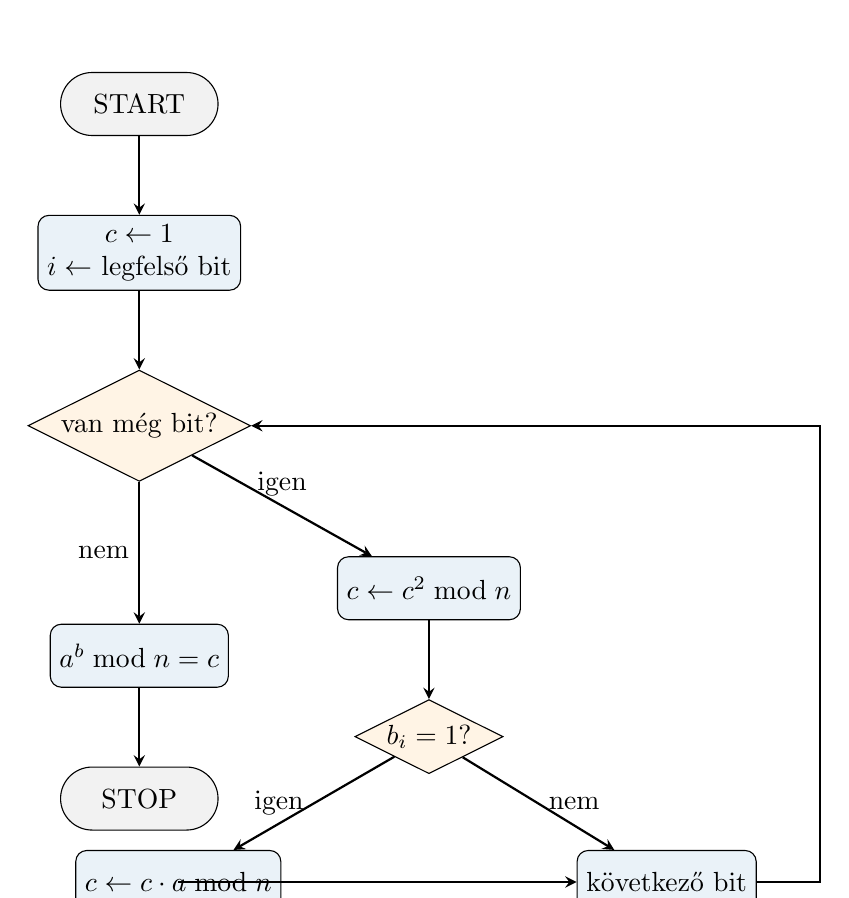
\begin{tikzpicture}[node distance=10mm]
  \node[terminator] (start) {START};
  \node[flow, below=of start] (init) {$c\leftarrow1$\\$i\leftarrow$ legfelső bit};
  \node[pred, below=of init] (endtest) {van még bit?};
  \node[flow, below right=13mm and 18mm of endtest] (square) {$c\leftarrow c^2\bmod n$};
  \node[pred, below=of square] (bittest) {$b_i=1$?};
  \node[flow, below left=12mm and 14mm of bittest] (mult) {$c\leftarrow c\cdot a\bmod n$};
  \node[flow, below right=12mm and 14mm of bittest] (next) {következő bit};
  \node[flow, below=18mm of endtest] (out) {$a^b\bmod n=c$};
  \node[terminator, below=of out] (stop) {STOP};
  \draw[arrow] (start) -- (init);
  \draw[arrow] (init) -- (endtest);
  \draw[arrow] (endtest) -- node[left] {nem} (out);
  \draw[arrow] (out) -- (stop);
  \draw[arrow] (endtest) -- node[above] {igen} (square);
  \draw[arrow] (square) -- (bittest);
  \draw[arrow] (bittest) -- node[left] {igen} (mult);
  \draw[arrow] (bittest) -- node[right] {nem} (next);
  \draw[arrow] (mult) |- (next);
  \draw[arrow] (next.east) -- ++(8mm,0) |- (endtest.east);
\end{tikzpicture}
\end{center}


\subsection{Pszeudókód}

\zvpseudocode[caption={Moduláris hatványozás négyzetre emeléssel},label={lst:zv04_modularis_hatvanyozas}]{src/code/zv04_modularis_hatvanyozas.pseudo}

A módszer csak $O(\log b)$ darab lépést végez, mert a kitevő bitjeinek száma $\lfloor\log_2 b\rfloor+1$.

\subsection{Példa}

A forrásanyagban szereplő tipikus példa:

\[
118^{2005}\bmod137.
\]

A kitevő bináris alakja:

\[
2005_{10}=11111010101_2.
\]

A négyzetre emeléses moduláris hatványozás eredménye:

\[
118^{2005}\equiv101\pmod{137}.
\]

A lényeg nem az, hogy $118^{2005}$ teljes értékét kiszámítjuk, hanem az, hogy minden köztes eredményt modulo $137$ szerint redukálunk.

\section{Fermat-tétel és Fermat-prímteszt}

\subsection{Fermat kis tétele}

Fermat kis tétele szerint ha $p$ prím és $a$ nem osztható $p$-vel, akkor

\[
a^{p-1}\equiv1\pmod p.
\]

Speciálisan, ha $1\leq a<p$, akkor biztosan $p\nmid a$, tehát a tétel alkalmazható.

\subsection{Fermat-féle prímteszt}

A Fermat-prímteszt ötlete:

\begin{enumerate}
  \item választunk egy $a$ alapot, például $a=2$;
  \item kiszámítjuk $a^{n-1}\bmod n$ értékét moduláris hatványozással;
  \item ha az eredmény nem $1$, akkor $n$ biztosan összetett;
  \item ha az eredmény $1$, akkor $n$ lehet prím, de ez nem teljes bizonyíték.
\end{enumerate}

Pszeudókód:

\zvpseudocode[caption={Fermat-prímteszt},label={lst:zv04_fermat_primteszt}]{src/code/zv04_fermat_primteszt.pseudo}

\subsection{A teszt értelmezése}

Ha a teszt azt mondja, hogy összetett, akkor az eredmény biztos. Ha azt mondja, hogy a szám valószínűleg prím, akkor hibázhat. Vannak olyan összetett számok, amelyek bizonyos alapokra teljesítik a Fermat-kongruenciát. Ezeket álprímeknek nevezzük. Különösen problémásak a Carmichael-számok, amelyek több alapra is prímnek tűnhetnek.

\begin{warningbox}
A Fermat-prímteszt gyors szűrő, nem abszolút bizonyító erejű prímteszt. Vizsgán fontos kiemelni: a negatív eredmény biztos összetettséget jelent, a pozitív eredmény csak valószínű prímséget.
\end{warningbox}

\subsection{Példák}

Vizsgáljuk $11$-et $a=2$ alappal:

\[
2^{10}=1024\equiv1\pmod{11}.
\]

Ez összhangban van azzal, hogy $11$ prím.

Vizsgáljuk $12$-t:

\[
2^{11}=2048\equiv8\pmod{12}.
\]

Mivel az eredmény nem $1$, ezért $12$ biztosan összetett.

\section{RSA algoritmus}

\subsection{Nyilvános kulcsú titkosítás alapgondolata}

A szimmetrikus titkosításnál ugyanaz a kulcs kell a titkosításhoz és a visszafejtéshez. Nyilvános kulcsú titkosításnál ezzel szemben két kulcs van:

\begin{itemize}
  \item \textbf{nyilvános kulcs}: bárki ismerheti, ezzel lehet titkosítani;
  \item \textbf{titkos kulcs}: csak a címzett ismeri, ezzel lehet visszafejteni.
\end{itemize}

Az RSA lényege, hogy a titkosítás és visszafejtés is moduláris hatványozás, a titkos kulcs meghatározása viszont a nyilvános adatokból a nagy számok faktorizálási nehézségére építve gyakorlatilag nehéz.

\subsection{RSA jelölések}

\begin{center}
\begingroup
\setlength{\tabcolsep}{4pt}
\begin{tabularx}{\textwidth}{>{\bfseries}L{0.17\textwidth}L{0.28\textwidth}X}
\toprule
Jelölés & Jelentés & Megjegyzés \\
\midrule
$p,q$ & két különböző nagy prímszám & Ezek titkos kiinduló adatok. Gyakorlati RSA-ban nagyon nagy, véletlenszerű prímeket használnak. \\
$n=pq$ & modulus & A nyilvános és a titkos kulcsban is szerepel. A biztonság alapja, hogy $n$ faktorizálása nagy számokra nehéz. \\
$\varphi(n)$ & Euler-féle függvény értéke & Két prím szorzatára $\varphi(n)=(p-1)(q-1)$. \\
$e$ & nyilvános kitevő & Úgy kell választani, hogy $1<e<\varphi(n)$ és $\operatorname{lnko}(e,\varphi(n))=1$. \\
$d$ & titkos kitevő & $d\equiv e^{-1}\pmod{\varphi(n)}$, vagyis $ed\equiv1\pmod{\varphi(n)}$. \\
$(e,n)$ & nyilvános kulcs & Ezzel bárki titkosíthat: $C\equiv M^e\pmod n$. \\
$(d,n)$ & titkos kulcs & Ezzel a címzett visszafejt: $M\equiv C^d\pmod n$. \\
\bottomrule
\end{tabularx}
\endgroup

\end{center}

\begin{center}
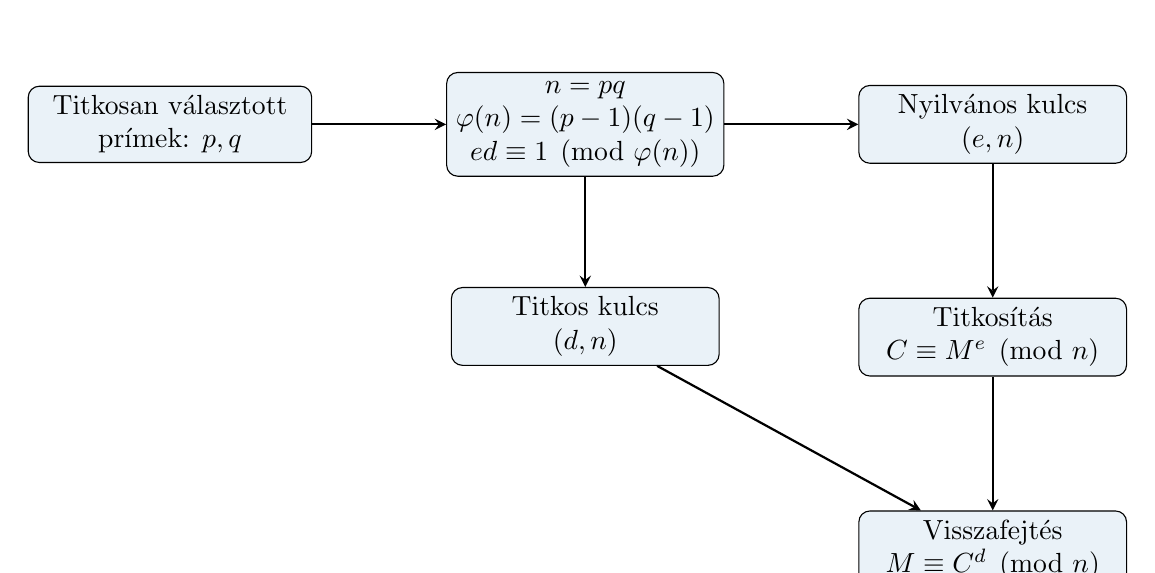
\begin{tikzpicture}[node distance=10mm]
  \node[flow, minimum width=36mm] (picks) {Titkosan választott\\prímek: $p,q$};
  \node[flow, right=17mm of picks, minimum width=35mm] (keys) {$n=pq$\\$\varphi(n)=(p-1)(q-1)$\\$ed\equiv1\pmod{\varphi(n)}$};
  \node[flow, right=17mm of keys, minimum width=34mm] (pub) {Nyilvános kulcs\\$(e,n)$};
  \node[flow, below=14mm of keys, minimum width=34mm] (priv) {Titkos kulcs\\$(d,n)$};
  \node[flow, below=17mm of pub, minimum width=34mm] (enc) {Titkosítás\\$C\equiv M^e\pmod n$};
  \node[flow, below=17mm of enc, minimum width=34mm] (dec) {Visszafejtés\\$M\equiv C^d\pmod n$};
  \draw[arrow] (picks) -- (keys);
  \draw[arrow] (keys) -- (pub);
  \draw[arrow] (keys) -- (priv);
  \draw[arrow] (pub) -- (enc);
  \draw[arrow] (enc) -- (dec);
  \draw[arrow] (priv) -- (dec);
\end{tikzpicture}
\end{center}


\subsection{Kulcsgenerálás}

Az RSA kulcsgenerálás lépései:

\begin{enumerate}
  \item választunk két különböző nagy prímet: $p$ és $q$;
  \item kiszámítjuk: $n=pq$;
  \item kiszámítjuk: $\varphi(n)=(p-1)(q-1)$;
  \item választunk egy $e$ számot úgy, hogy $1<e<\varphi(n)$ és $\operatorname{lnko}(e,\varphi(n))=1$;
  \item meghatározzuk $d$-t úgy, hogy $ed\equiv1\pmod{\varphi(n)}$;
  \item a nyilvános kulcs: $(e,n)$;
  \item a titkos kulcs: $(d,n)$.
\end{enumerate}

A $d$ érték kiszámítása pontosan multiplikatív inverz keresése:

\[
d=e^{-1}\pmod{\varphi(n)}.
\]

Ehhez a kibővített euklideszi algoritmust használjuk.

\subsection{Titkosítás és visszafejtés}

Legyen $M$ az üzenet számmá alakított blokkja, ahol $0\leq M<n$. A titkosítás:

\[
C\equiv M^e\pmod n.
\]

A visszafejtés:

\[
M\equiv C^d\pmod n.
\]

Mindkét műveletet moduláris hatványozással célszerű végezni.

\subsection{Kis számpélda}

A következő példa oktatási célú, nem biztonságos méretű számokkal dolgozik.

Legyen:

\[
p=11,
\]

\[
q=29.
\]

Ekkor:

\[
n=pq=11\cdot29=319,
\]

\[
\varphi(n)=(p-1)(q-1)=10\cdot28=280.
\]

Válasszuk:

\[
e=3.
\]

Mivel

\[
\operatorname{lnko}(3,280)=1,
\]

az $e$ megfelelő. A titkos kitevő:

\[
d\equiv3^{-1}\pmod{280}.
\]

A kibővített euklideszi algoritmusból:

\[
d=187,
\]

mert

\[
3\cdot187=561\equiv1\pmod{280}.
\]

Ezért:

\[
\text{nyilvános kulcs}=(3,319),
\]

\[
\text{titkos kulcs}=(187,319).
\]

Titkosítsuk az

\[
M=100
\]

üzenetet:

\[
C\equiv100^3\pmod{319}=254.
\]

Visszafejtés:

\[
M\equiv254^{187}\pmod{319}=100.
\]

Tehát a visszafejtés visszaadja az eredeti üzenetet.

\subsection{Miért működik?}

A részletes bizonyítás a moduláris számelméletre és Euler-tételre épül. Vizsgaszinten a lényeg:

\begin{itemize}
  \item $d$ úgy van választva, hogy $ed\equiv1\pmod{\varphi(n)}$;
  \item ezért létezik olyan $k$, hogy $ed=1+k\varphi(n)$;
  \item a titkosítás után a visszafejtés lényegében $M^{ed}$ kiszámítása modulo $n$ szerint;
  \item a megfelelő számelméleti tétel miatt ez visszaadja $M$-et modulo $n$ szerint.
\end{itemize}

\subsection{Biztonsági alapgondolat}

Az RSA nyilvános kulcsában benne van $n$ és $e$. Ha valaki meg tudná határozni $p$-t és $q$-t az $n=pq$ felbontásból, akkor ki tudná számítani $\varphi(n)$-t, majd abból $d$-t. Ezért a biztonság gyakorlati alapja az, hogy nagy $n$ esetén a faktorizálás nehéz.

\begin{warningbox}
Az RSA matematikai vázlata egyszerű, de a gyakorlati, biztonságos használat nem merül ki ebben. Valódi rendszerekben megfelelő kulcsméretre, véletlenszám-generálásra, padding eljárásra és protokollszintű védelemre is szükség van. Vizsgán azonban általában a fenti alapalgoritmus és a hozzá tartozó számelméleti háttér a lényeg.
\end{warningbox}

\section{Kapcsolatok az egyes algoritmusok között}

A tétel részei egymásra épülnek:

\begin{enumerate}
  \item az euklideszi algoritmus gyorsan kiszámítja az lnko-t;
  \item a kibővített euklideszi algoritmus megadja az lnko lineáris kombinációs alakját;
  \item ebből eldönthető és megoldható a lineáris kongruencia;
  \item speciális esetként kiszámítható a multiplikatív inverz;
  \item az RSA titkos kitevője ilyen multiplikatív inverz;
  \item a moduláris hatványozás teszi gyorssá a Fermat-tesztet, az RSA titkosítást és az RSA visszafejtést;
  \item a Fermat-teszt a nagy prímek keresésének egyik egyszerű, valószínűségi eszköze.
\end{enumerate}

Egy tömör képletben:

\[
\text{Euklidesz} \Rightarrow \text{inverz} \Rightarrow \text{RSA-kulcs},
\]

\[
\text{moduláris hatványozás} \Rightarrow \text{Fermat-teszt és RSA-műveletek}.
\]

\section{Tipikus vizsgakérdések és válaszvázlatok}

\subsection{Mi az euklideszi algoritmus lényege?}

Az, hogy az $\operatorname{lnko}(a,b)$ értéke nem változik, ha $(a,b)$ helyett $(b,a\bmod b)$ párral folytatjuk. Ezt addig ismételjük, amíg a második szám nulla nem lesz. Az aktuális első szám az lnko.

\subsection{Miben több a kibővített euklideszi algoritmus?}

Nemcsak $d=\operatorname{lnko}(a,b)$ értékét számolja ki, hanem olyan $x,y$ egész számokat is, amelyekre $d=ax+by$. Ez a lineáris kombináció szükséges a kongruenciaegyenletek és az inverzek meghatározásához.

\subsection{Mikor oldható meg az $ax\equiv b\pmod n$ kongruencia?}

Pontosan akkor, ha $d=\operatorname{lnko}(a,n)$ osztja $b$-t. Ha $d\mid b$, akkor $d$ darab alapmegoldás van modulo $n$ szerint. Ha $d\nmid b$, akkor nincs megoldás.

\subsection{Mikor létezik $a^{-1}\pmod n$?}

Akkor és csak akkor, ha $\operatorname{lnko}(a,n)=1$. Ilyenkor a kibővített euklideszi algoritmusból kapott $x$ együttható modulo $n$ szerint az inverz.

\subsection{Miért gyors a moduláris hatványozás?}

Mert nem $b$ darab szorzást végez, hanem a kitevő bináris alakja alapján halad, ezért csak $O(\log b)$ darab négyzetre emelésre és legfeljebb ugyanennyi szorzásra van szükség. Minden lépésben modulo $n$ szerint redukál, így a számok mérete kezelhető marad.

\subsection{Mit állít Fermat kis tétele?}

Ha $p$ prím és $p\nmid a$, akkor $a^{p-1}\equiv1\pmod p$. Erre épül a Fermat-prímteszt: ha a kongruencia nem teljesül, akkor a szám biztosan összetett; ha teljesül, akkor a szám csak valószínűleg prím.

\subsection{Mik az RSA kulcsgenerálás fő lépései?}

Két nagy prímet választunk: $p,q$. Kiszámítjuk $n=pq$ és $\varphi(n)=(p-1)(q-1)$. Választunk $e$-t úgy, hogy relatív prím legyen $\varphi(n)$-hez. Ezután kiszámítjuk $d=e^{-1}\pmod{\varphi(n)}$ értékét. A nyilvános kulcs $(e,n)$, a titkos kulcs $(d,n)$.

\subsection{Miért kapcsolódik az RSA az euklideszi algoritmushoz?}

Az RSA titkos kitevője az $e$ multiplikatív inverze modulo $\varphi(n)$ szerint. Ezt az inverzet a kibővített euklideszi algoritmussal lehet hatékonyan kiszámítani.

\section{Rövid összefoglalás}

\begin{summarybox}
A számelméleti algoritmusok alapja a maradékos osztás és a kongruencia. Az euklideszi algoritmus gyorsan meghatározza két szám legnagyobb közös osztóját, a kibővített változat pedig Bézout-együtthatókat is ad. Ezekkel megoldhatók a lineáris kongruencia egyenletek, és kiszámítható a multiplikatív inverz. A moduláris hatványozás a nagy kitevőjű hatványokat hatékonyan számolja modulo $n$ szerint. A Fermat-prímteszt gyors, de nem tévedhetetlen valószínűségi prímteszt. Az RSA a fenti elemeket kapcsolja össze: a kulcsgenerálás inverzszámítást, a titkosítás és visszafejtés moduláris hatványozást használ.
\end{summarybox}

\section{Vizsgán gyorsan elmondható feleletvázlat}

\begin{enumerate}
  \item A tétel alapja az oszthatóság, a maradékos osztás és a kongruencia: $a\equiv b\pmod n$ pontosan akkor, ha $n\mid(a-b)$.
  \item Az $\operatorname{lnko}(a,b)$ a legnagyobb közös osztó. Ha értéke $1$, akkor $a$ és $b$ relatív prímek.
  \item Az euklideszi algoritmus a $\operatorname{lnko}(a,b)=\operatorname{lnko}(b,a\bmod b)$ összefüggést ismétli, amíg a maradék nulla nem lesz.
  \item A kibővített euklideszi algoritmus $d=\operatorname{lnko}(a,b)$ mellett $x,y$ értékeket is ad úgy, hogy $d=ax+by$.
  \item Az $ax\equiv b\pmod n$ lineáris kongruencia pontosan akkor oldható meg, ha $\operatorname{lnko}(a,n)$ osztja $b$-t.
  \item Az $a^{-1}\pmod n$ multiplikatív inverz pontosan akkor létezik, ha $\operatorname{lnko}(a,n)=1$.
  \item A moduláris hatványozás négyzetre emeléssel és szorzással $O(\log b)$ lépésben számolja $a^b\bmod n$ értékét.
  \item Fermat kis tétele: ha $p$ prím és $p\nmid a$, akkor $a^{p-1}\equiv1\pmod p$.
  \item A Fermat-prímteszt negatív eredménye biztos összetettséget jelent, pozitív eredménye csak valószínű prímséget.
  \item RSA-ban $n=pq$, $\varphi(n)=(p-1)(q-1)$, $d=e^{-1}\pmod{\varphi(n)}$, a nyilvános kulcs $(e,n)$, a titkos kulcs $(d,n)$.
\end{enumerate}

\end{document}
